\documentclass[a4paper, 14pt]{article}
\usepackage{fontspec, extsizes, geometry, setspace, titlesec, fancyhdr, graphicx, float, setspace, caption, csquotes, color, listings, booktabs, subcaption, enumitem, indentfirst}
\newcommand{\bigcell}[2]{\begin{tabular}{@{}#1@{}}#2\end{tabular}}
\usepackage[russian, english, ukrainian]{babel}
\usepackage[dotinlabels]{titletoc}
\tolerance=1
\emergencystretch=\maxdimen
\hyphenpenalty=10000
\hbadness=10000
\usepackage[normalem]{ulem}
\renewcommand{\ULdepth}{1.8pt}
\bibliographystyle{gost-numeric}
\usepackage[backend=biber, bibstyle=gost-numeric]{biblatex}
\addbibresource{paper.bib}
\setmainfont[Ligatures=TeX]{Times New Roman}
\geometry{a4paper,total={170mm,257mm},left=1.7cm,top=2cm,bottom=2cm,right=1.7cm}
\def\changemargin#1#2{\list{}{\rightmargin#2\leftmargin#1}\item[]}\let\endchangemargin=\endlist % удобная команда
\makeatletter\newcommand\Dotfill{\leavevmode\leaders\hb@xt@0.65em{\hss.\hss}\hfill}\makeatother % удобная команда
\let\stdsection\section\renewcommand\section{\newpage\stdsection} % Новая секция -> новая страница
\addto\captionsenglish{\renewcommand{\figurename}{Рис.}} % Подпись картинок
\titleformat{\section}[display]{\filcenter}{\bfseries{РОЗДІЛ \thesection}}{0pt}{\bfseries \MakeUppercase} % Изменение заголовка всех разделов
\renewcommand{\thesubsection}{\arabic{section}.\arabic{subsection}} % Чиним номер подраздела
\titleformat{\subsection}{}{\hspace{21pt}\bfseries \thesubsection.\hspace{10mm}}{0pt}{\bfseries}{} %чиним название подраздела 
\titleformat{\subsubsection}{}{\hspace{21pt}\thesubsubsection. }{0pt}{}{} %чиним название подподраздела 
\captionsetup{labelsep=period} % "Рис. 1." вместо "Рис. 1:"
\fancyhf{}\renewcommand{\headrulewidth}{0pt}\newcommand{\changefont}{\fontsize{14}{14}\selectfont}\fancyhead[R]{\changefont \thepage}\fancypagestyle{plain}{\fancyhf{}\fancyhead[R]{\changefont \thepage}\renewcommand{\headrulewidth}{0pt}\renewcommand{\footrulewidth}{0pt}}\pagestyle{fancy} %номер страницы справа сверху на всех страничках [это ужас]
\linespread{1.25} %#1
\renewcommand{\contentsname}{ЗМІСТ} %изменяем название странички с содержанием
\def\numberline#1{#1. } % Фикс чтобы названия не налезали друг на друга в содержании
\titlecontents{section}[0cm]{\normalfont}{РОЗДІЛ \thecontentslabel. \MakeUppercase}{\MakeUppercase}{\Dotfill \contentspage} % точки в содержании
\titlecontents{subsection}[0.625cm]{\normalfont}{\thecontentslabel.}{}{\Dotfill \contentspage} % точки в содержании
\titlecontents{subsubsection}[1.25cm]{\normalfont}{\thecontentslabel. }{}{\Dotfill \contentspage} % точки в содержании
\newcommand{\RNum}[1]{\uppercase\expandafter{\romannumeral #1\relax}}
\definecolor{dkgreen}{rgb}{0,0.6,0}
\definecolor{gray}{rgb}{0.5,0.5,0.5}
\definecolor{mauve}{rgb}{0.58,0,0.82}
\graphicspath{{./images/}}
\setlist[itemize]{leftmargin=32pt}
\setlist[enumerate]{leftmargin=32pt}
\lstset{frame=tb, language=Java,  aboveskip=3mm,  belowskip=3mm,  showstringspaces=false,  columns=flexible,  basicstyle={\small\ttfamily},  numbers=none,  numberstyle=\tiny\color{gray},  keywordstyle=\color{blue},  commentstyle=\color{dkgreen},  stringstyle=\color{mauve},  breaklines=true,  breakatwhitespace=true, tabsize=2
}
\lstset{moredelim=[is][\textit]{[*}{*]}}
\counterwithin{figure}{section}
\counterwithin{table}{section}
\begin{document}
% Титулка
\thispagestyle{empty}
\begin{spacing}{1}
\begin{center}
Міністерство освіти і науки України \\
Департамент науки і освіти Харківської обласної державної адміністрації \\
Комунальний заклад «Харківська обласна Мала академія наук \\ Харківської обласної ради» \\
\end{center}\par\null\par
\begin{center}
Відділення комп'ютерних наук\\
Секція: технології програмування
\end{center}\par\null\par
\begin{center}
\textbf{МЕТОД ПОШУКУ ТА УСУНЕННЯ ПОВТОРЮВАНИХ
ЧАСТИН У ПОЧАТКОВОМУ КОДІ ПРОГРАМНОГО ЗАБЕЗПЕЧЕННЯ}
\end{center}\par\null\par\null
\begin{changemargin}{9.75cm}{0cm}
Роботу виконав:\\ 
\textbf{Човпан Ігор Сергійович},\\
учень 11 класу Харківського\\
навчально-виховного комплексу\\
№45 «Академічна гімназія»\\
Харківської міської ради\\
Харківської області
\end{changemargin}\par
\begin{changemargin}{9.75cm}{0cm}
Науковий керівник:\\
\textbf{Руккас Кирило Маркович},\\
професор кафедри теоретичної\\
та прикладної інформатики\\
механіко-математичного\\
факультету Харківського\\
національного університету\\
ім. В.Н. Каразіна, доктор\\
технічних наук, доцент\\
\vspace*{\fill}\end{changemargin}
\begin{center}
Харків -- \the\year{}
\end{center}\end{spacing}

% Тези
\pagebreak
\noindent
\begin{center}
\textbf{
АНОТАЦІЯ \\
МЕТОД ПОШУКУ ТА УСУНЕННЯ ПОВТОРЮВАНИХ ЧАСТИН \\ 
У ПОЧАТКОВОМУ КОДІ ПРОГРАМНОГО ЗАБЕЗПЕЧЕННЯ
}
\end{center}
\textbf{Човпан Ігор Сергійович}; 11 клас; Харківське територіальне відділення МАН України; Харківський навчально-виховний комплекс №45 «Академічна гімназія»; Харківської міської ради Харківської області; \\ \textbf{Руккас Кирило Маркович}; професор кафедри теоретичної та прикладної інформатики механіко-математичного факультету Харківського національного університету ім. В.Н. Каразіна, доктор технічних наук, доцент. \\
\par Серед розробників програмного забезпечення практика копіювання та вставки коду є досить поширеною. Вона може призводити до катастрофічних наслідків при обслуговуванні програмного забезпечення. Копії стають джерелом помилок та вразливостей, для їх підтримки потрібно забагато ресурсів.
Через досить велику відносну кількість копій у початковому коді, пошук та їх усунення є важливою задачею.
\par Існує досить багато методів пошуку копій, але в кожного є свої недоліки. Наприклад, у методах, використовуючих абстрактне синтаксичне дерево, головною перешкодою є завелика алгоритмічна складність. Евристики, що застосовуються при усуненні цієї проблеми, є досить неефективними.
Метою роботи є аналіз існуючих методів знаходження повторюваних частин, створення нового алгоритму знаходження й усунення копій, що має задовільні ефективність та складність.
\par Був створений новий алгоритм, який визначає потенційні місця знаходження копій, перетворює код у список виразів, обчислює максимум функції кількості потенційно видалених рядків коду від відрізка виразів, відмічає та замінює відповідні виразам частини коду на виклик новоствореної функції.
\par Новий метод знаходить та видаляє клони у великих проєктах (Apache OpenOffice, Tomcat, тощо) за досить малий час, має задовільні показники влучності та повноти.
За результатами експерименту продемонстровано, що алгоритм є кращим.
\par \textbf{Ключові слова:} програма, код, копії, усунення, копіювання, вставка, якість коду

\tableofcontents %генерация содержания
\section*{\textbf{ВСТУП}}
\addcontentsline{toc}{section}{Вступ} %добавляем страницу ВСТУП в содержание
\textbf{Актуальність роботи}.
Серед розробників програмного забезпечення практика копіювання та вставки коду є досить поширеною. Не дивлячись на те, що це може бути корисним та зручною навичкою у короткостроковій перспективі, подібна практика призводить до катастрофічних наслідків при обслуговуванні програмного забезпечення. \\ Так, наприклад, будь яке удосконалення чи усунення помилки потрібно буде робити для кожної копії, що робиться далеко не завжди. Через це істотно збільшується кількість потенційних вразливостей та помилок у коді, на підтримку програмного забезпечення великих розмірів потрібно значно більше ресурсів. \\
Досліди показують, що доволі велику частину від початкового коду проєкту займають копії (у середньому 5-10\% \cite{Baxter98}). \\
Через це, пошук та усунення повторюваних частин у початковому коді є важливою задачею. \\
Існує досить багато методів пошуку копій, але в кожного є свої недоліки. Наприклад, у методах, використовуючих абстрактне синтаксичне дерево, головною перешкодою є завелика алгоритмічна складність. Евристики, що застосовуються при усуненні цієї проблеми, є досить неефективними. У роботі \cite{Baxter98} асимптотика створеного алгоритма залежить квадратично від кількості рядків у початковому коді. Це призводить до того, що для пошуку клонів у проєктах відносно невеликого розміру потрібно занадто багато часу. \cite{Sager06} 
\par\textbf{Мета роботи} -- аналіз існуючих методів знаходження повторюваних частин у початковому коді програмного забезпечення та створення нового алгоритму знаходження і усунення копій, що має задовільні ефективність та час, потрібний для обчислення на проєктах великого розміру.
\par \textbf{Завдання дослідження}:
\begin{itemize}
	\item виділити 4 основних типи повторюваних частин;
	\item проаналізувати методи знаходження повторюваних частин, виділити переваги та недоліки кожного з методів;
	\item створити новий алгоритм, який усуває недоліки розглянутих методів;
	\item зробити порівняння між новим алгоритмом та існуючими методами.
\end{itemize}
\par\textbf{Об’єкт дослідження} -- процеси знахождення повторюваних частин у програмному коді.
\par\textbf{Предмет дослідження} -- математичні та програмні моделі знаходження повторюваних частин у програмному коді.
\par\textbf{Особистий внесок автора}. Робота виконана автором самостійно.
\par\textbf{Практичне значення}. Результати дослідження можуть бути використані для вирішення проблеми збільшення кількості помилок та вразливостей у програмі, а також при розробці нових алгоритмів виявлення та усунення копій у початковому коді програмного забезпечення.
\newpage
\section{Характеристика існуючих методів знаходження повторюваних частин у коді}
\label{sec:characteristics}
\par Щоб проаналізувати методи знахождення повторюваних частин, треба визначити, що таке повторювана частина.
\par Уважатимемо дублікатом фрагмент, який є ідентичним з іншим фрагментом коду. Тоді повторювана частина коду -- фрагмент, в якого є дублікати.
\par Визначемо основні види повторюваних частин.
\subsection{Основні види повторюваних частин}
Як зазначено у роботах \cite{Gautam16}, \cite{Dang15} та \cite{Thummalapenta10}, виділяється 4 головних типи повторюваних частин. 
\begin{itemize}
\item \RNum{1} тип -- повна копія без модифікацій, окрім пробілів та коментарів;
\begin{figure}[!htb]
\centering
\begin{minipage}[t]{.45\textwidth}
\begin{lstlisting}[frame=none]
double xx = Math.cos(angle);
double yy = Math.sin(angle);
xx*=2;
yy*=2;	
if (xx>PI)
	xx = 2*PI-xx;
if (yy>PI)
	yy = 2*PI-yy;
\end{lstlisting}
\end{minipage}
\begin{minipage}[t]{.45\textwidth}
\begin{lstlisting}[frame=none]
double xx = Math.cos(angle);
// of course using math package!!
double yy = Math.sin(angle);
xx *= 2;
yy *= 2;	
if ( xx > PI)
//That is VERY important statement!
	xx = 2 * PI - xx; 
if (yy > PI)
	yy = 2 * PI - yy;
\end{lstlisting}
\end{minipage}
\caption{Приклад копії \RNum{1} типу на мові Java}
\end{figure} \\
\item \RNum{2} тип -- синтаксично однакова копія, змінюються лише назви змінних, назв функцій, тощо;
\begin{figure}[!htb]
\centering
\begin{minipage}[t]{.45\textwidth}
\begin{lstlisting}[frame=none]
void func(double angle) {
	double xx = Math.cos(angle);
	double yy = Math.sin(angle);
	xx*=2;
	yy*=2;	
	if (xx>PI)
		xx = 2*PI-xx;
	if (yy>PI)
		yy = 2*PI-yy;
	write(xx);
}
\end{lstlisting}
\end{minipage}
\begin{minipage}[t]{.45\textwidth}
\begin{lstlisting}[frame=none]
void veryImportantFunc(double ang){
	double aa = Math.cos(ang);
	double bb = Math.sin(ang);
	aa*=2;
	bb*=2;	
	if (xx>PI_CONST)
		aa = 2*PI_CONST-aa;
	if (yy>PI_CONST)
		bb = 2*PI_CONST-bb;
	writeToFile(aa);
}
\end{lstlisting}
\end{minipage}
\caption{Приклад копії \RNum{2} типу}
\end{figure} \\
\item \RNum{3} тип -- копія з подальшими змінами; доданими, зміненими або видаленими інструкціями;
\begin{figure} 
\centering
\begin{minipage}[t]{.45\textwidth}
\begin{lstlisting}[frame=none]
void func(double angle) {
	double xx = Math.cos(angle);
	double yy = Math.sin(angle);
	double PI = Math.acos(-1);
	xx*=2;
	yy*=2;	
	if (xx>PI)
		xx = 2*PI-xx;
	if (yy>PI)
		yy = 2*PI-yy;
	write(xx);
}
\end{lstlisting}
\end{minipage}
\begin{minipage}[t]{.45\textwidth}
\begin{lstlisting}[frame=none]
void doCalc(double ang){
	double bb = Math.sin(ang);
	double aa = Math.cos(ang);
	print("before"+aa);
	aa*=2;
	if (xx>PI_CONST)
		aa = 2*PI_CONST-aa;
	bb*=2;	
	if (yy>PI_CONST)
		bb = 2*PI_CONST-bb;
	print(aa);
}
\end{lstlisting}
\end{minipage}
\caption{Приклад копії \RNum{3} типу}
\end{figure} \\
\item \RNum{4} тип -- частина, що робить ідентичні обчислювання, але синтаксично імплементована інакше.
\begin{figure}
\centering
\begin{minipage}[t]{.45\textwidth}
\begin{lstlisting}[frame=none]
int fibonacci(int n) {
	int sum1=0, sum2=1;
	for (int i=2; i<=n; i++){
		int sum3 = sum3+sum2;
		sum1 = sum2;
		sum2 = sum3;
	}
	return sum2;
}
\end{lstlisting}
\end{minipage}
\begin{minipage}[t]{.45\textwidth}
\begin{lstlisting}[frame=none]
int[] mem = new int[...];
int fib(int n) {
	if (mem[n]!=0)
		return mem[n];
	if (n<2)
		return 1;
	mem[n] = fib(n-1)+fib(n-2);
	return mem[n];
}
\end{lstlisting}
\end{minipage}
\caption{Приклад копії \RNum{4} типу}
\end{figure} \\
\end{itemize}
\subsection{Основні методи пошуку повторюваних частин}
Існує багато прийомів, що використовуються для пошуку повторюваних частин у початковому коді програмного забезпечення.

Перелічим основні методи пошуку:
\begin{itemize}
	\item пошук збігу рядків початкового коду; 
	\item використання токенів;
	\item метод порівняння функцій;
	\item застосування графа програмних залежностей;
	\item метод порівняння дерев.
\end{itemize}
Далі визначимо усі переваги і недоліки кожного з методів.

\subsubsection{Пошук збігу рядків початкового коду}
Обчислюється ступінь схожості для кожної пари рядків за допомогою відстані Левенштейна. Емпірично встановлюється мінімальна величина, за якої вважається, що 2 рядки є копіями одна одної

Переваги цього методу:  
\begin{itemize}
\item добре знаходить копії \RNum{1} типу;
\item невеликий час виконання порівняно з іншими методами;
\item підтримка будь-якої мови программування.
\end{itemize}

Недоліки методу:
\begin{itemize}
\item велика кількість хибнонегативних результатів;
\item нестійкість до різних "шумів": коментарів, змінених назв функцій або змінних, тобто неможливість знайти дублікати \RNum{2} та \RNum{3} типу. 
\item Не враховуються особливості мови програмування.
\end{itemize}
Прикладом використання є програма PMD.
\subsubsection{Використання токенів}
Початковий код розбивається на токени, при пошуці порівнюються послідовності токенів.
Головною перевагою цього методу є стійкість до переформатування початкового коду, зміні назв змінних.
Недоліком є те, що токенізатори враховують тільки базові особливості мови програмування, тому багато послідовностей, які вважаються копіями, насправді самі по собі не мають сенсу. \cite{Koschke06}
\begin{figure}[h!]
\centering
\begin{minipage}[t]{.275\textwidth}
\begin{lstlisting}[frame=none]
return x;
void func(int y) {
  y++;
\end{lstlisting}
\end{minipage}
\begin{minipage}[t]{.275\textwidth}
\begin{lstlisting}[frame=none]
return a;
void myFunc(int b) {
  b++;
\end{lstlisting}
\end{minipage}
\begin{minipage}[t]{.35\textwidth}
\begin{lstlisting}[frame=none]
void,myFunc,(,int,b,),{,b,++,;
\end{lstlisting}
\end{minipage}
\caption{Частини коду, що вважатимуться копіями; приклад розбиття коду на токени}
\end{figure}
Прикладом використання такого методу є програма CCFnderX. 
\subsubsection{Метод порівняння функцій}
За допомогою парсера мови програмування знаходять усі функції в початковому коді. Далі усі ці функції порівнюються між собою або за допомогою спеціально обраної <<поганої>> геш-функції, або за допомогою обчислення коефіцієнту схожості (наприклад, коеф. Жаккара).
Метод гарно знаходить збіги між різними функціями, розпізнаються копії \RNum{1}-\RNum{3} типу, проте він не може знайти повторювани частини всередині функції.
Прикладом використання є \cite{Yang18}.
\subsubsection{Застосування графа програмних залежностей}
Згідно з \cite{Ferrante87}, граф програмних залежностей (далі просто граф) -- представлення програми як графа, у якому кожна вершина - інструкція в програмі, а також зв'язані з цією інструкцією оператори та операнди; ребрамивв такому графі є дані, від яких залежить виконання цієї інструкції та умови, за яких ця інструкція виконається.
\begin{figure}[h]
    \centering
    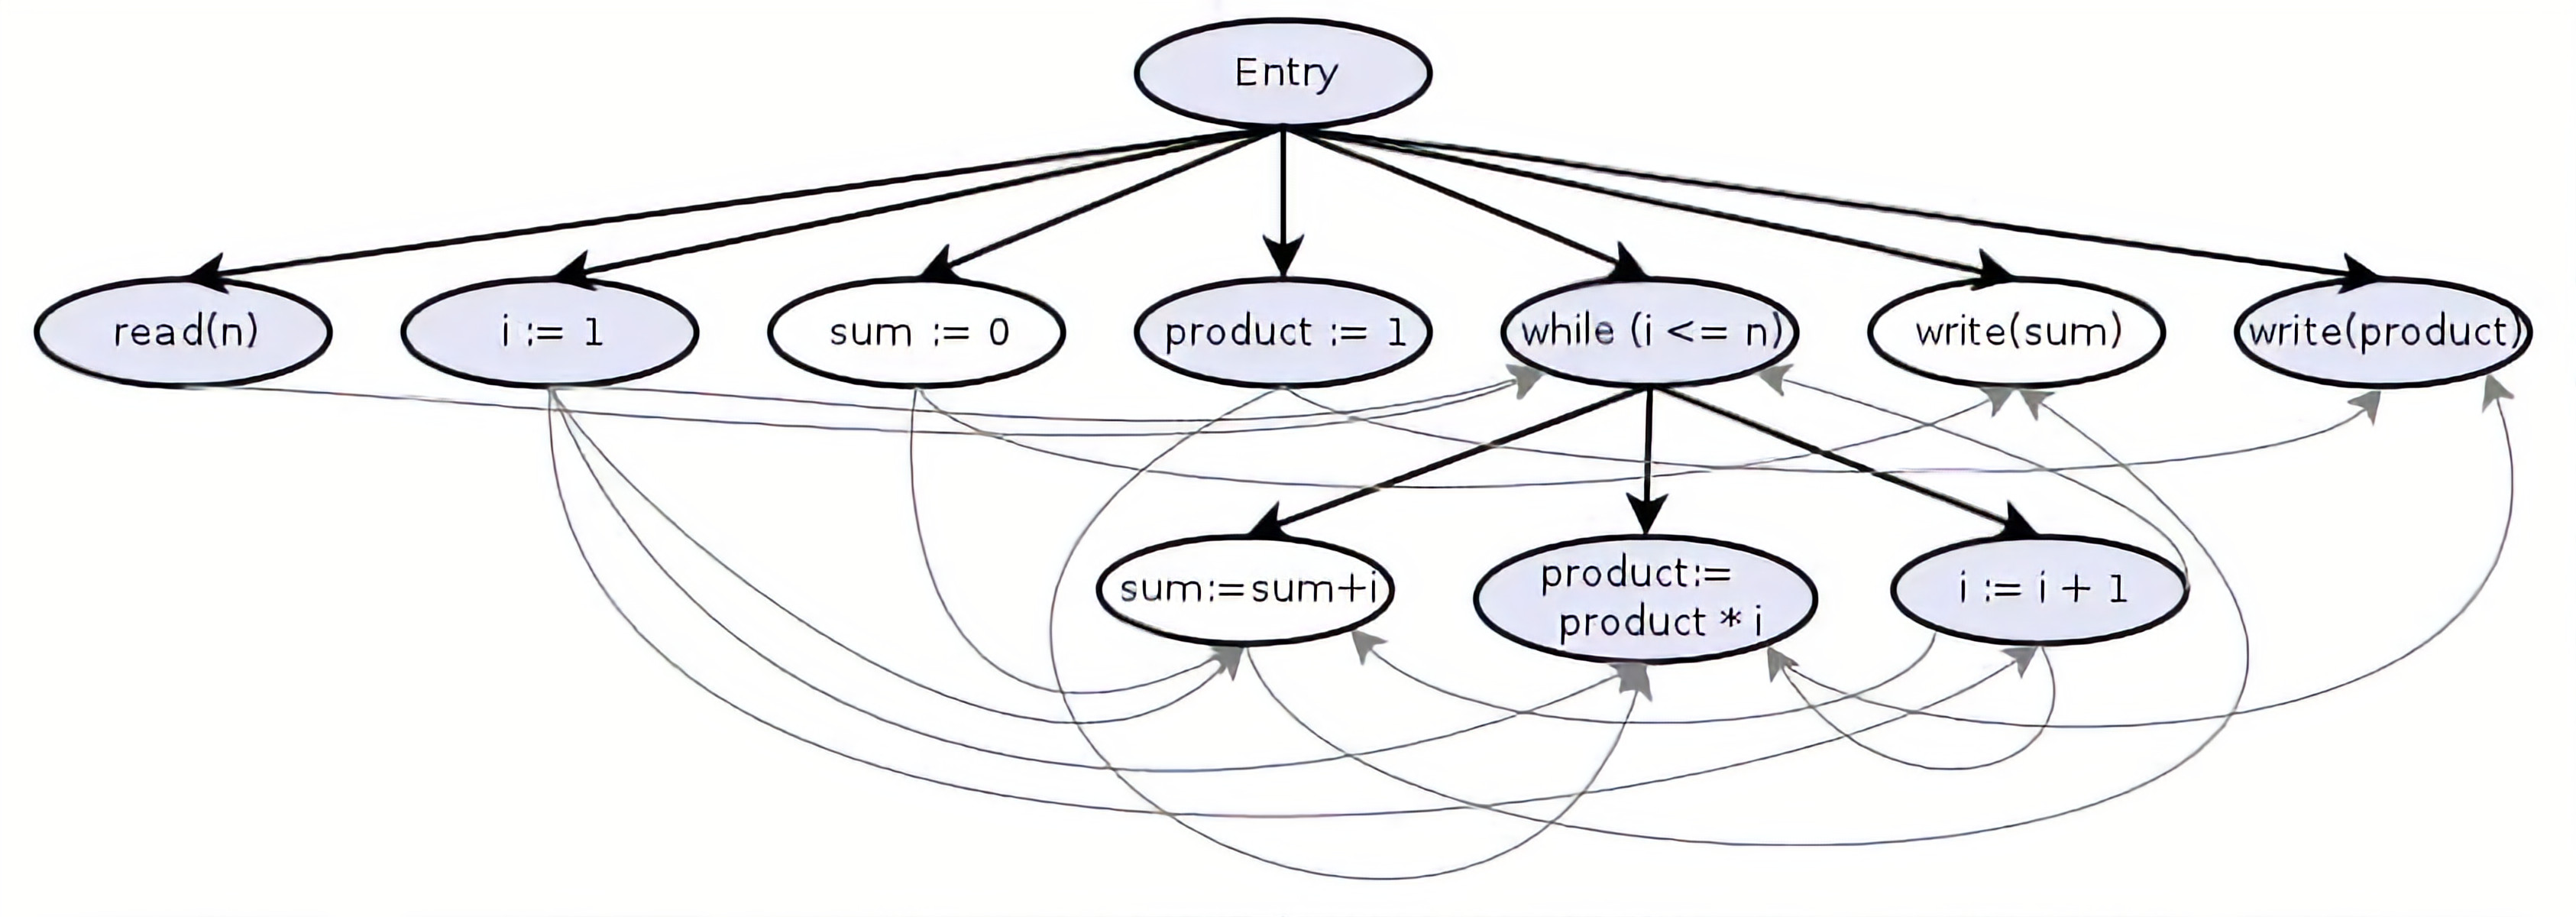
\includegraphics[width=0.75\textwidth]{pdg-example}
    \caption{Приклад графа програмних залежностей \cite{pdg-example}}
    \label{fig:pdg-example}
\end{figure} 
Дві частини програми вважаються ідентичними, якщо їх графи ізоморфні.
Головною перевагою є те, що цей граф не залежить від переставлення інструкцій, зміни назв функцій, тощо; не залежить від аспектів реалізації.
Недоліки методу:
\begin{itemize}
\item Дуже довгий час роботи, оскільки завдання пошуку ізоморфних підграфів є NP-повною, і може бути вирішена за поліноміальний час тільки для планарних графів, що не обов'язково виконується для графа програмних залежностей.
\item Такий метод не зможе знайти дублікати у коді, який не виконується у загальному випадку, оскільки у граф додаються лише виконані інструкції.
\end{itemize}
Приклад використання: \cite{Liu06}.
\subsubsection{Метод порівняння дерев}
У цьому методі використовуються абстрактні синтаксичні дерева (АСД). Згідно з \cite{wiki:ast}, абстрактне синтаксичне дерево -- позначене й орієнтоване дерево, в якому внутрішні вершини співставлені з відповідними операторами мови програмування, а листя з відповідними операндами.
\begin{figure}[h!]
    \centering
    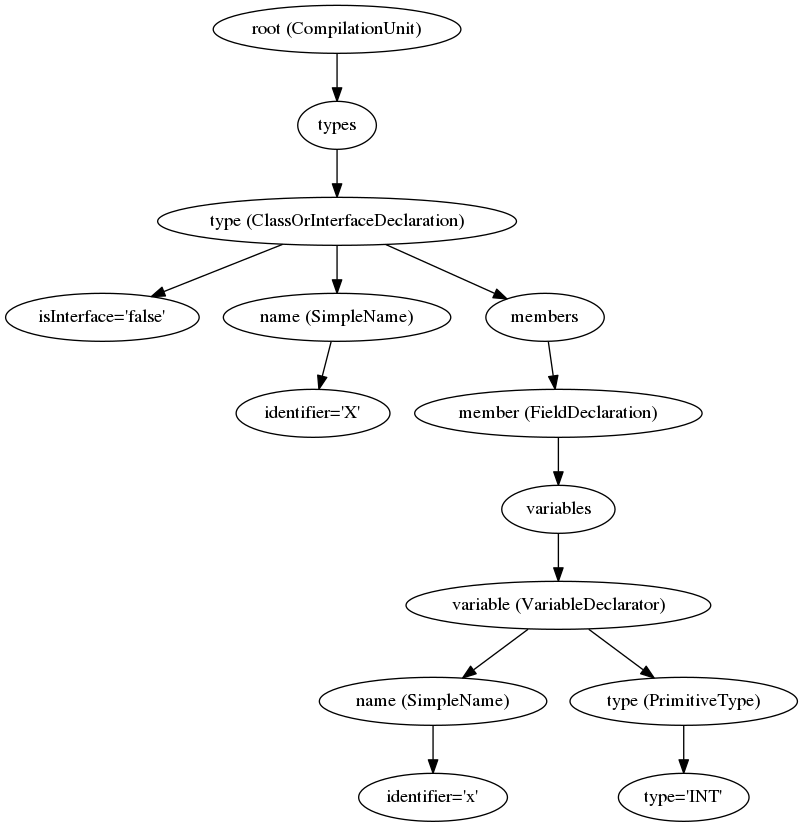
\includegraphics[width=0.5\textwidth]{ast-example}
    \caption{Приклад абстрактного синтаксичного дерева \cite{ast-example}}
    \label{fig:ast-example}
\end{figure}\\
Щоб визначити, чи є частина коду копією іншої частини, знаходять відповідні їм піддерева, а далі ці піддерева порівнюються між собою. \\
Підходів до порівяння піддерев досить багато. Так, наприклад, у роботі \cite{Sager06} усі піддерева, що відповідають класам у початковому коді, порівнюються один з одним за допомогою обчислення відстані між деревами. Автор зазначає, що цей метод є найточнішим порівняно з іншими, але має дуже довгий час роботи. Наприклад, код плагінів \verb|org.eclipse.compare-plug-in|, що складався зі 114 класів перевірявся на копії більше ніж годину. \\
У роботі \cite{Baxter98} теж стверджується, що алгоритм знахождення відстані між деревами має занадто велику складність обчислення, тому автором був запропонований інший підхід. Усі піддерева гешуються за допомогою вибраної <<поганої>> геш-функції та розподіляються у $B$ бакетів, де $B \approx N/10$. 
Далі кожне піддерево порівнюється лише з піддеревами з цього ж бакету за формулою: $$\frac{2*S}{2*S+L+R}.$$ $S$ -- кількість однакових вершин у обох піддеревах, $L$ -- кількість вершин, що присутні лише в першому піддереві, $R$ -- кількість вершин, що є тільки в другому піддереві. \\
Отже, головними перешкодами до використання цього методу є:
\begin{itemize} 
\item Великі час роботи та алгоритмічна складність; \cite{Ain19}
\item Досить низький відсоток знайдених копій через використання додаткових евристик. \cite{Dang15}
\end{itemize}
Далі буде запропоновано новий підхід, що значно зменшить час роботи, необхідний для знаходження копій, та, у той же час, збільшить ефективність їх знаходження.
\section{Метод пошуку та видалення копій з використанням алгоритму порівняння графів}
Алгоритм складається із 4 кроків:
\begin{enumerate}[label={{\arabic*})}]
\item парсинг коду та перетворення його в абстрактне синтаксичне дерево;
\item визначення частин коду, які має сенс порівнювати;
\item знаходження повторюваних частин;
\item перетворення знайденого результату до конкретних елементів у коді.
\end{enumerate}
Далі опишемо детальніше кожен крок.
\subsection{Парсинг коду}
Компілятор практично будь-якої мови програмування на якомусь кроку перетворює код у абстрактне синтаксичне дерево. Для простоти будемо працювати з кодом, написаним мовою програмування \verb|Java|. Щоб перетворити код на абстрактне синтаксичне дерево, використаємо \verb|JavaParser|. Алгоритм не складно змінити для підтримки будь-якої іншої мови програмування.
\subsection{Визначення частин коду, які підлягають порівнянню}
У загальному випадку структура коду в об'єктно-оріентованих мовах програмування виглядає таким чином: \\
\begin{figure}[h!]
\begin{lstlisting}[frame=none, xleftmargin=.3\textwidth]
import com.google.tools;
class X {
	int a=0;
	X(int a, int b)	{
		this.a = a;
	}
	void incrementAndPrint()	{
		a++;
	}
}
\end{lstlisting}
\caption{Приклад коду в об'єктно-орієнтованих мовах програмування}
\end{figure} 
\par Можна визначити головні елементи практично кожної програми, а саме:
\begin{itemize}
\item підключення інших пакетів, бібліотек;
\item декларування класу та його елементи (поля);
\item декларування функцій та обчислення якогось результату.
\end{itemize}
\par Порівнянню і подальшому опрацюванню підлягають лише ті частини коду, які можна винести до іншої функції.
Цими елементами є тільки ствердження у функціях.
\par Пояснемо на прикладі:
\begin{figure}[h!]
\begin{lstlisting}[frame=none, xleftmargin=.3\textwidth]
import com.google.tools;
class X {
	int a=0;
	X(int a)	{
		[*this.a = a;*]
	}
	void incrementAndPrint()	{
		[*a++;
		print(a);*]
	}
}
\end{lstlisting}
\caption{Приклад коду}
\end{figure}
\par Курсивом виділені фрагменти коду, що будуть далі опрацьовані.
\par Визначимо вираз (<<expression>>) як найменшу неподільну операцію та параметр до цієї операції. Будь-яке велике обчислення можна розбити на вирази.
\par У операціях розгалуження вважатимемо виразами лише додаткові умови у них, але не самі операції.
\par Блок -- непорожня послідовність виразів, укладених між фігурними дужками та впорядкованих за порядком обходу алгоритма DFS у абстрактному синтаксичному дереві.
\par Алгоритм розбиває код на блоки таким чином, що вміст одного блоку не зустрічається в іншому. В кожного виразу є свої координати: перша координата($x$) -- номер блоку, в якому є цей вираз, друга координата($y$) -- знаходження виразу в блоці.
\begin{figure}[h!]
\centering
\begin{minipage}{.4\textwidth}
\begin{lstlisting}[frame=none]
void func(){
	int x = 10;
	x = x+1;
	while (x>3){
		System.out.println(x*2);
		x--;
	}
}
\end{lstlisting}
\end{minipage}
\begin{minipage}{.5\textwidth}
\begin{lstlisting}[frame=none]
[int x = 10;, x = x + 1;, x > 3, System.out.println(x * 2);, x--;]
\end{lstlisting}
\end{minipage}
\caption{Приклад розбиття коду на вирази в блоці}
\end{figure}
\par Порівнянню з іншою послідовністю підлягає будь-яка послідовність виразів, що йдуть поспіль та знаходяться в одному блоці.
\subsection{Знаходження повторюваних частин}
У загальному випадку в клонах є доволі багато ідентичних виразів. Для простоти будемо вважати, що клони починаються з ідентичного виразу. У майбутньому планується підтримка випадку, коли клони починаються не з ідентичного виразу.
\par Знаходження повторюваних частин працює таким чином:
\begin{itemize}
\item для кожного виразу обчислити геш-функцію для кожного виразу;\\
у геш-функції враховуються усі типи кожного з вершин АСД, що лежать нижче, ніж відповідна вершина до цього виразу; типи буквальних виразів (наприклад, \verb|123.0f| це тип \verb|float|, \verb|"123"| -- тип \verb|String|);
\item{створити асоціативний масиву, де ключем є геш, а значенням є список координат усіх виразів;}
\item{перетворити асоціативний масив на масив зі списків до кожного ключа;}
\item{відсортувати масив за зростанням наступної функції: $$f(list)=\max_{\forall expr \in list}{expr_{y}} $$ \\
Це потрібно для того, щоб потенційний відрізок не обмежувався іншим, вже відміченим як копією, відрізком;}
\item{для кожного списка координат з цього масива: 
\begin{enumerate}[label={{\arabic*})}]
\item{знайти максимум функції: $$F(len)=(len-2*T-1)*goodGraphs-len-2$$
$len$ -- довжина відрізка виразів. При обчисленні функції створюється дерево структури відрізка виразів, де кожний вираз зустрічається один раз. \\
Один вираз є батьком (<<parent>>) іншого, якщо перший вираз є частиною операції розгалуження, а другий вираз знаходиться в тілі цієї операції. \\
У кожної вершини є свій напис (<<label>>). Вважатимемо написом кожної вершини тип відповідного виразу. \\
\begin{figure}[h]
    \centering
    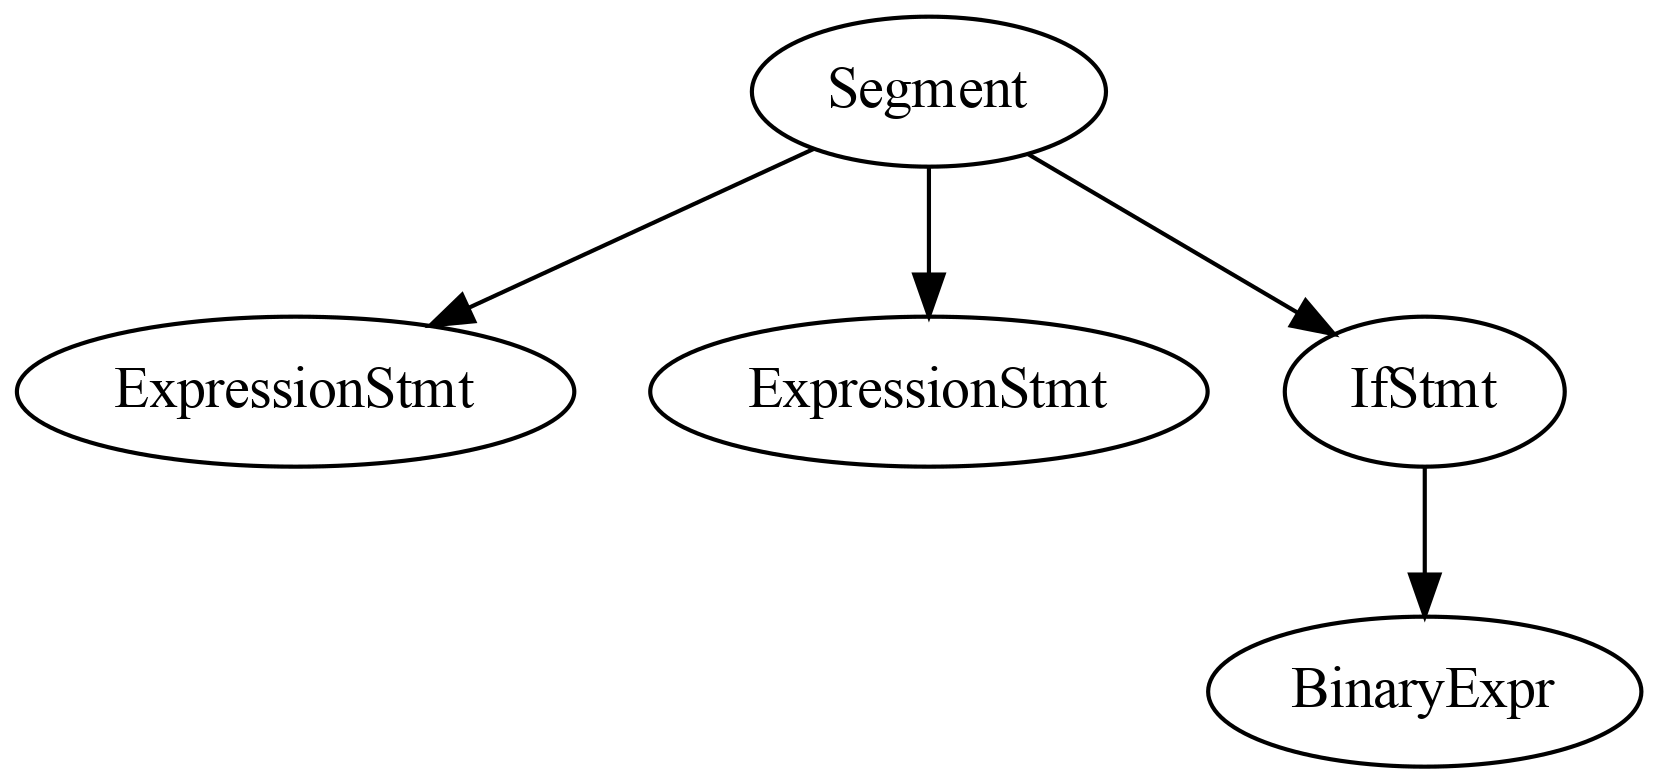
\includegraphics[width=0.75\textwidth]{function_graph_example}
    \caption{Приклад створеного графу}
    \label{fig:}
\end{figure} \\
$goodGraphs$ -- кількість графів (окрім першого), для яких відстань зміни графа до першого є меншою за константу $T$\footnote{Відстань зміни графа обчислюється за допомогою алгоритму APTED. \cite{Pawlik15}\cite{Pawlik16}}. \\
Відстань зміни графа вимірюється за 3 параметрами: 
\begin{itemize}
\item вартість видалення вершини (дорівнює $0.5$);
\item вартість зміни <<напису>> вершини (дорівнює $1$);
\item вартість вставки вершини (дорівнює $0.5$).
\end{itemize}
Для кращого знаходження дублікатів \RNum{3} типу, вартості видалення і вставки зменшені, 
тоді вартість переставлення виразу буде такою ж, як і вартість зміни <<напису>>.\\
Слід зазначити, що $$D(F)=[3, maxPotentialLen] \backslash \forall len: $$
$$\exists piece, piece_y \geq start_y+len, piece \in varusages, $$
$$\exists decl, start_{y} \leq decl_{y} < start_{y}+len, $$
$$decl \in declarations, decl_{var}=piece_{var};$$
$$maxPotentialLen = min(exprCount, y_{nearest})-start_y,$$ де:
\begin{itemize} 
\item $3$ -- константа, обрана емпірічно, щоб відрізки меншої довжини не вважалися клонами, бо вони не мають сенсу для програміста;
\item $maxPotentialLen$ -- максимально можлива довжина відрізка;
\item $start$ -- почтаковий вираз відрізка;
\item $varusages$ -- множина усіх використань змінних у цьому відрізку;
\item $declarations$ -- множина усіх декларацій змінних у цьому відрізку;
\item $decl_{var}$, $piece_{var}$ -- імена відповідних змінних;
\item $exprCount$ -- кількість виразів у блоці;
\item $y_{nearest}$ -- y-координата найближчого виразу-клона.
\end{itemize}
Додаткова умова додана, щоб не було таких випадків, коли декларація використованої змінної вже відсутня.
$F(len)$ -- приблизна кількість рядків у коді, що будуть зекономлені.
$$F(len) = len*goodGraphs-goodGraphs-2*T*goodGraphs-len-2,$$ 
де:
\begin{itemize}
\item $len*goodGraphs$ -- приблизна початкова кількість рядків коду;
\item $goodGraphs$ -- кількість потрібних викликів нової функції, кожен виклик зазвичай займає 1 рядок;
\item $2*T*goodGraphs$ -- приблизна кількість рядків коду, потрібного для врахування усіх відмінностей між послідовностями виразів;
\item $len$ -- приблизна кількість рядків коду, що є повністю ідентичним між усіма послідовностями;
\item $2$ -- кількість рядків, необхідна щоб записати функцію у коді.
\end{itemize}
$$F(len) = len*goodGraphs-goodGraphs-2*T*goodGraphs-len-2$$
$$F(len) = (len-1)*goodGraphs-2*T*goodGraphs-len-2$$
$$F(len) = (len-2*T-1)*goodGraphs-len-2;$$
}
\item якщо кількість відрізків більша за $1$ і $F(len)>0$, то усі вирази у відрізку відмітити як вирази-клони.
$F(len)$ повинно бути більше ніж 0, бо в інакшому випадку у сгенерованому коді буде більше рядків, а це не має сенсу.
\end{enumerate}
}
\end{itemize}
\subsection{Перетворення на послідовність фрагментів у коді}
Попереднім кроком були знайдені усі вирази-клони, але їх ще потрібно перетворити у послідовність фрагментів, бо самі по собі вирази показують лише уривки з початкового коду.   
\begin{figure}[h!]
\centering
\begin{minipage}{.5\textwidth}
\begin{lstlisting}[frame=none]
[xx == 466.0f,xx == 143.0f,xx == 466.0f,xx++;,xx == 143.0f,xx++;]
\end{lstlisting}
\end{minipage}
\begin{minipage}{.4\textwidth}
\begin{lstlisting}[frame=none]
if (xx==466.0f || xx==143.0f) {
  if (xx==466.0f)
		xx++;
	else if (xx==143.0f)
		xx++;
}	
\end{lstlisting}
\end{minipage}
\caption{Приклад послідовності виразів-клонів та відповідна їм частина коду}
\end{figure} \\
Зробимо перетворення наступним чином: оберемо усі вершини в абстрактному синтаксичному дереві (АСД), для яких
$$\exists piece, LCA(son, piece_{ast}) = son,$$
де:
\begin{itemize}
\item $son$ -- син закріпленої за блоком вершини у АСД, 
\item $piece$ -- вираз, 
\item $piece_{ast}$ -- відповідна виразу вершина у АСД.
\end{itemize}
Таким чином для послідовності виразів-клонів закріплені вершини в абстрактному синтаксичному дереві.
У подальшому називатимемо ці вершини інструкціями.
\subsection{Алгоритм видалення клонів}
Для видалення списка повторюваних частин коду об'єднаємо їх у функцію за алгоритмом. \\
\begin{enumerate}
\item Кожна повторювана частина коду є списком інструкцій. \\
Тілом функції буде найбільша спільна підпослідовність цих списків.
\item Виконання кожної іншої інструкції, що не увійшла до найбільшої спільної підпослідовності, обернемо в оператор \verb|if|.
Умовою цього оператору стане параметр функції типу \verb|boolean|.
\item Додати до усіх використаних змінних, полів, викликів функцій з іншої частини коду назву класу.
\item Усі буквальні вирази, що є у найбільшій спільній підпослідовності та не є однаковими для усіх відповідних інструкцій, замінимо на параметр функції. Тип параметру може бути визначений за допомогою бібліотеки \verb|JavaParser|.
\item Для кожної повторюваної частини замінити першу інструкцію в списку на виклик нової функції, інші інструкції видалити.
\item Нову функцію записати у файл \verb|Copied.java|.
\end{enumerate}
\newpage
\begin{figure}[h!]
\centering
\begin{minipage}{.45\textwidth}
\begin{lstlisting}[frame=none]
static final double PI = 3.1415;
static void veryImportantFunction()
{
	double xx = Math.cos(PI/2)-Math.sin(PI/2);
	double yy = Math.sin(PI/2)+Math.cos(PI/2);
	if (xx==456.0f || xx==123.0f){
		if (xx==456.0f)
			xx++;
		else if (xx==123.0f)
			xx++;
	}
	xx*=2;
	yy*=2;
	System.out.println(xx+" "+yy);
}
\end{lstlisting}
\end{minipage}
\begin{minipage}{.45\textwidth}
\begin{lstlisting}[frame=none]
static final double PI = 3.1415;
static void superComputing()
{
	double aa = Math.cos(PI/2)-Math.sin(PI/2);
	double bb = Math.sin(PI/2)+Math.cos(PI/2);
	if (aa==345.0f || aa==0f){
		if (aa==345.0f)
			aa++;
		else if (aa==0.0f)
			aa++;
	}
	aa*=2;
	bb*=2;
	System.out.println(aa+" "+bb);
}
\end{lstlisting}
\end{minipage}
\caption{Приклад коду до виконання алгоритмів}
\end{figure}

\begin{figure}[h!]
\centering
\begin{subfigure}[t]{0.4\textwidth}
\begin{lstlisting}[frame=none]
static final double PI = 3.1415;
static void veryImportantFunction() {
  Copied.
    veryImportantFunction(456.0f, 123.0f, 456.0f, 123.0f);
}
static void superComputing() {
  Copied.
    veryImportantFunction(345.0f, 0f, 345.0f, 0.0f);
}
\end{lstlisting}
\caption{Змінений код початкових функцій}
\end{subfigure}
\begin{subfigure}[t]{0.5\textwidth}
\begin{lstlisting}[frame=none]
static final double PI = 3.1415;
static void veryImportantFunction(Double literalXx, Double literalXx2, Double literalXx3, Double literalXx4) {
  double xx = Math.cos(Main.PI / 2) - Math.sin(Main.PI / 2);
  double yy = Math.sin(Main.PI / 2) + Math.cos(Main.PI / 2);
  if (xx == literalXx || xx == literalXx2) {
    if (xx == literalXx3)
      xx++;
    else if (xx == literalXx4)
      xx++;
  }
  xx *= 2;
  yy *= 2;
	System.out.println(xx+" "+yy);
}
\end{lstlisting}
\caption{Нова функція, що була створена алгоритмом}
\end{subfigure}
\caption{Приклад роботи обох алгоритмів: знаходження та видалення клонів}
\end{figure} 
\section{Аналіз ефективності запропонованого методу}
Порівняємо запропонований алгоритм з іншими методами на наступному обладнанні:
\begin{itemize}
\item процесор -- \verb|Intel Core i5-8250U|, 1.60Ггц;
\item оперативна пам'ять -- 8 Гб;
\item операційна система -- \verb|Windows 10|.
\end{itemize} 
Зазвичай порівняння виконується за 3 основними параметрами: 
\begin{itemize}
\item влучність (<<precision>>, \cite{wiki:precisionrecall}). Інструмент повинен детектувати якомога менше хибно-позитивних клонів. Влучність обчислюється як відношення правильно знайдених пар клонів до усіх знайдених інструментом пар клонів;
\item повнота (<<recall>>, \cite{wiki:precisionrecall}). Інструмент має коректно знаходити більшість пар клонів серед можливих (тобто відмічених людиною). Повнота обчислюється як відношення кількості коректно знайдених пар клонів до кількості відмічених людиною пар клонів;
\item час роботи інструменту.
\end{itemize}
\par Використання інших характеристик так чи інакше потребує ручної перевірки, що не є об'єктивним через потенційну упередженість.
\subsection{Порівняння з іншими методами за влучністю та повнотою}
\par Для підрахунку перших двох параметрів необхідно з'ясувати, які пари клонів потрібно вважати правильними. \\ 
Це можна зробити двома способами: перевіряючи на реальних проєктах знайдені інструментами пари клонів (\cite{Bellon07}), або порівнюючи результат роботи інструменту зі згенерованими парами. \par 
Як показано в роботі \cite{Roy18}, використання першого варіанту проблематично, оскільки в такому разі ручна перевірка неминуча. Відмічається, що присутня значна непослідовність у визначенні типів клонів. У роботі \cite{Charpentier15} також зазначається на розбіжності висновків незалежних суддів у визначенні правильності знайдених пар клонів. \par
Приведені вище недоліки практично ліквідовані в бенчмарку <<\verb|BigCloneBench|>> \cite{Svajlenko14}, який використовує автоматично сгенеровану базу даних клонів <<\verb|IJaDataset|>>, для якої були узяті реалізації визначених алгоритмів з подальшою їх зміною декількома способами: видалення рядка, коментування рядка, тощо. На його основі був створений фреймворк <<\verb|BigCloneEval|>> для спрощення перевірки інструментів знаходження клонів, який і будемо використовувати для підрахунку параметрів влучності та повноти. \par
Для порівняння з новим алгоритмом обрані наступні програми:
\begin{itemize}
\item \verb|CCFinderX|;
\item \verb|PMD|;
\item \verb|CloneDR|.
\end{itemize}
Ці програми є реалізаціями різних методів, описаних у розділі \ref{sec:characteristics}.
Отримані наступні результати:
\begin{table}[ht]
\centering
\caption*{\hspace{14.33cm} \textit{Таблиця 3.1} \\\null\\ \centering\textbf{Порівняння інструментів знаходження клонів за влучністю та повнотою}}
 \begin{tabular}{| c | c | c |} 
 \hline
 Назва інструменту & Влучність & Повнота \\ [0.5ex] 
 \hline
 \verb|CCFinderX| & 0.57 & 0.5 \\
 \hline
 \verb|PMD| & 0.48 & 0.58 \\
 \hline
 \verb|CloneDR| & 0.82 & 0.47 \\
 \hline
 Новий алгоритм & 0.76 & 0.55 \\ [1ex]
 \hline
\end{tabular} 
\end{table}
\par Як бачимо, новий алгоритм є значно влучнішим, ніж інструменти \verb|CCFinderX|, \verb|PMD| менш влучним ніж \verb|CloneDR|, проте в цього інструменту повнота є меншою. \par
Повнота нового алгоритму є більшою, ніж у всіх програм, окрім \verb|PMD|, в якого влучність є значно меншою, а повнота -- лише трохи більшою. \par
Таким чином ефективність нового алгоритму за показниками влучності та повноти є задовільною.
\subsection{Порівняння часу роботи}
На відміну від повноти та влучності час роботи є параметром, який можна оцінювати на коді реальних проєктів. \par
Порівняємо час роботи алгоритму з іншими програмами на початковому коді 16 проєктів:
\begin{itemize}
\item \verb|Eclipse| ($\sim$20000 рядків \verb|Java|-коду);
\item \verb|Bval| ($\sim$30000 рядків);
\item \verb|Attic-onami| ($\sim$40000 рядків);
\item \verb|DnsJava| ($\sim$40000 рядків коду);
\item \verb|Any23| ($\sim$50000 рядків);
\item \verb|Gorra| ($\sim$70000 рядків);
\item \verb|JSPWiki| ($\sim$90000 рядків);
\item \verb|OpenNLP| ($\sim$100000 рядків);
\item \verb|JHotDraw| ($\sim$120000 рядків);
\item \verb|Maven| ($\sim$120000 рядків);
\item \verb|Oodt| ($\sim$160000 рядків);
\item \verb|Juddi| ($\sim$180000 рядків);
\item \verb|ArgoUML| ($\sim$300000 рядків);
\item \verb|JFreeChart| ($\sim$300000 рядків);
\item \verb|Tomcat| ($\sim$600000 рядків);
\item \verb|OpenOffice| ($\sim$800000 рядків).
\end{itemize}
Отримані результати наведені на рисунках \ref{fig:graphd1} та \ref{fig:graphd2}. \newpage
\begin{figure}[h]
    \centering
    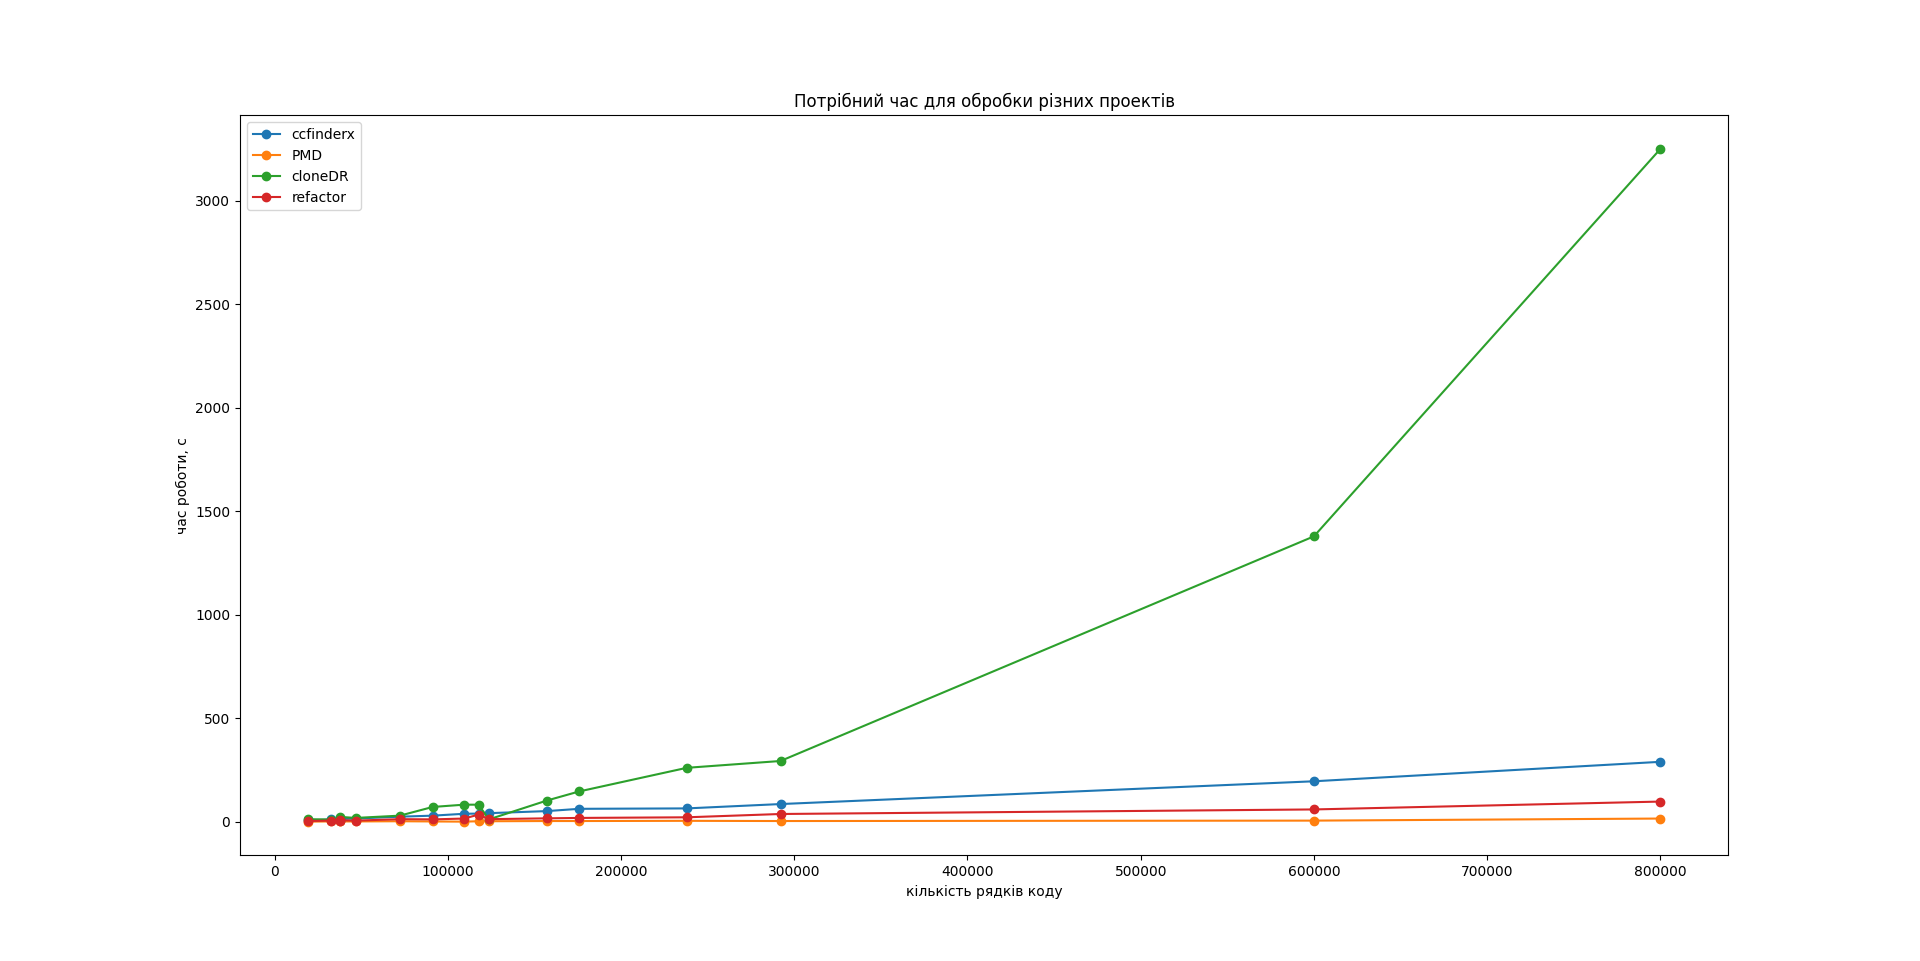
\includegraphics[width=0.9\textwidth]{graph1}
		\caption{Залежність часу виконання від кількості рядків коду \label{fig:graphd1}}
\end{figure} \hfill \par
\begin{figure}[h]
    \centering
    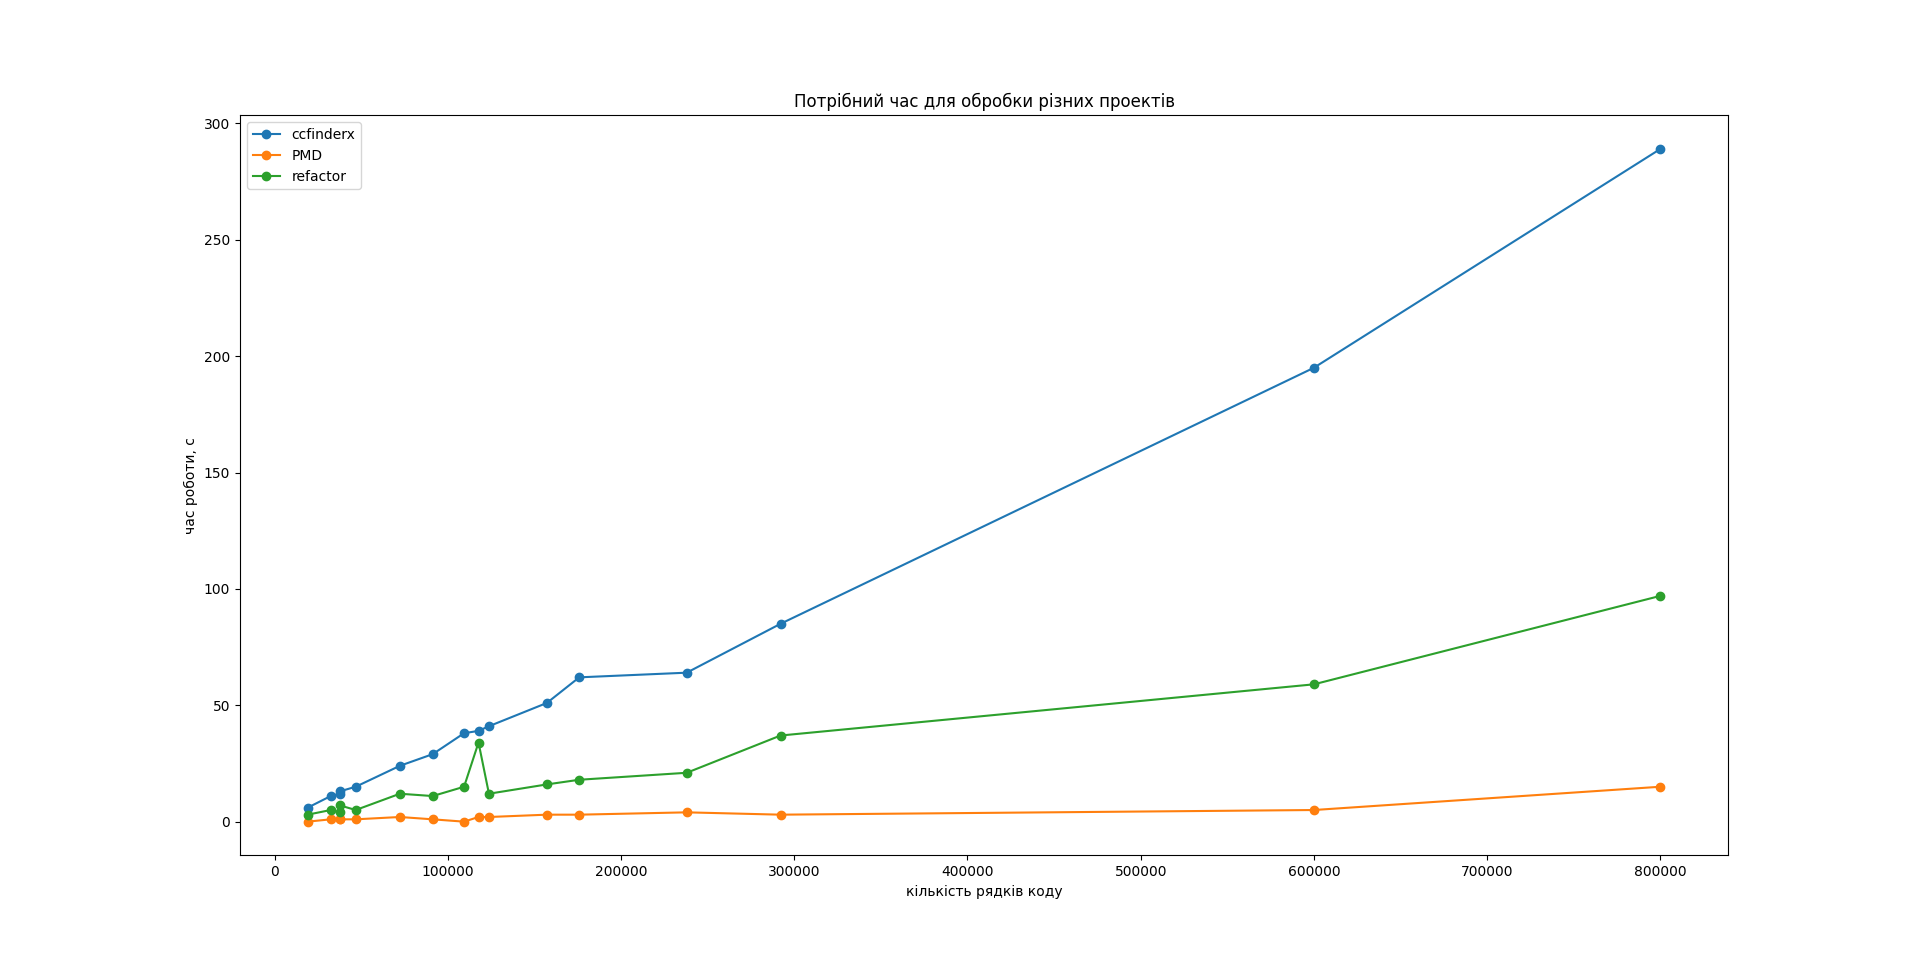
\includegraphics[width=0.9\textwidth]{graph2}
    \caption{\centering Залежність часу виконання інструментів (окрім CloneDR) від кількості рядків коду \label{fig:graphd2}}
\end{figure}
За наведеними вище даними, можна побачити, що новий алгоритм є значно швидшим, ніж \verb|CCFinderX| та \verb|CloneDR| (у $3$ та $30$ разів відповідно), але трохи повільнишим, ніж \verb|PMD|. \par
Зазначимо, що системи дуже великого розміру оброблюються швидко: проєкт із $\sim$800000 рядками коду оброблюється менш, ніж за 2 хвилини. \par
Час роботи, потрібний алгоритму для обчислення результату, є задовільним.
\section*{\textbf{Висновки}}
\addcontentsline{toc}{section}{Висновки}
Виділені 4 головних типи повторюваних частин:
\begin{itemize}
\item \RNum{1} тип -- повна копія практично з відсутніми модифікаціями;
\item \RNum{2} тип -- змінюються лише назви змінних, функцій, класів;
\item \RNum{3} тип -- копія із доданими, зміненими, або видаленими інструкціями, зміненими назвами об'єктів;
\item \RNum{4} тип -- копія, що значно відрізняється синтаксично, але робить ідентичні обчислювання.
\end{itemize}
\par Були проаналізовані наступні методи знаходження повторюваних частин у початковому коді програмного забезпечення:
\begin{itemize}
\item пошук збігу рядків початкового коду;
\item використання токенів;
\item метод порівняння функцій;
\item застосування графа програмних залежностей;
\item метод порівняння дерев.
\end{itemize} 
\par Виявлені основні переваги і недоліки кожного з методів. \par 
Створений новий алгоритм, який усуває недоліки методу порівняння дерев, а саме:
\begin{itemize}
\item надто великі час роботи та алгоритмічна складність;
\item досить низький коефіцієнт повноти через використання додаткових евристик.
\end{itemize}
\par Зроблено порівняння між новим алгоритмом та існуючими методами за 3 основними показниками: влучністю, повнотою та часом роботи. \par
Продемонстровано, що новий метод є кращим: має задовільні показники влучності та повноти (0.76 та 0.55 відповідно); може використовуватись на системах дуже великого розміру: проєкт з $\sim$800000 рядками коду оброблюється менш, ніж за 2 хвилини.
\newpage
\addcontentsline{toc}{section}{Список використаних джерел}
\printbibliography[title={\textbf{список використаних джерел}}]
\titleformat{\section}[display]{\raggedleft}{\bfseries{РОЗДІЛ \thesection}}{0pt}{} % Изменение заголовка всех разделов
\section*{Додаток А}
\counterwithout{figure}{section}
\setcounter{figure}{0}    
\addcontentsline{toc}{section}{Додатки}
\begin{figure}[h]
    \centering
    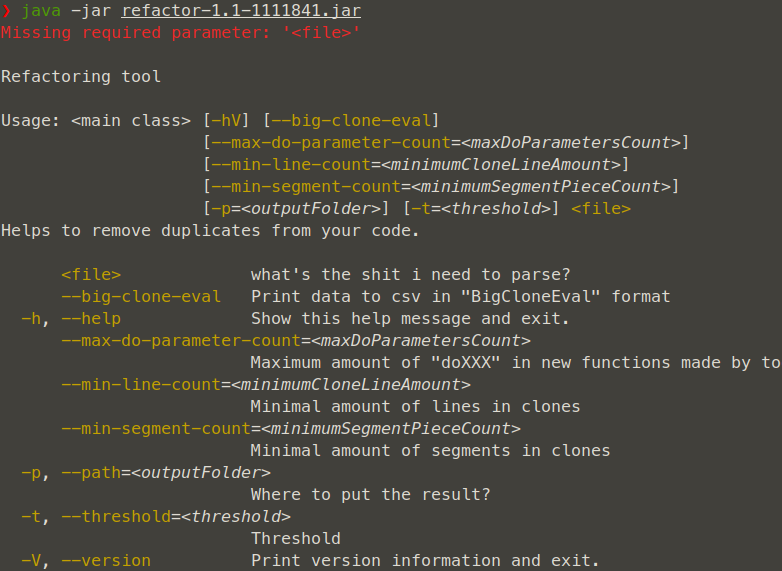
\includegraphics[width=\textwidth]{add1}
    \caption{\centering Список параметрів програми}
\end{figure} \hfill \\
\section*{Додаток Б}
\begin{figure}[h]
    \centering
    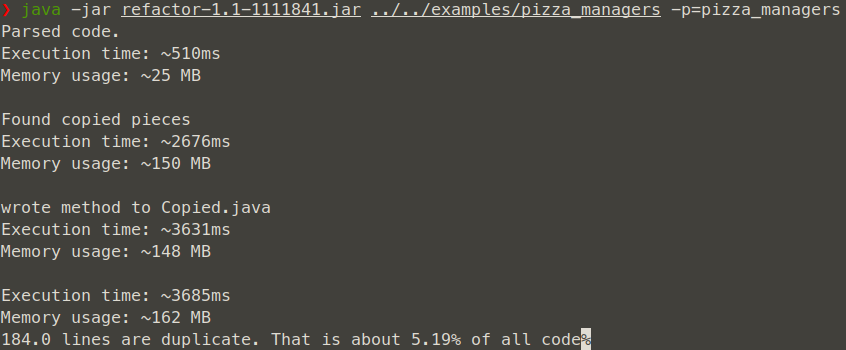
\includegraphics[width=\textwidth]{add2}
    \caption{\centering Приклад обробки проєкту програмою}
\end{figure} \hfill \\
\section*{Додаток В}
\begin{figure}[h]
    \centering
    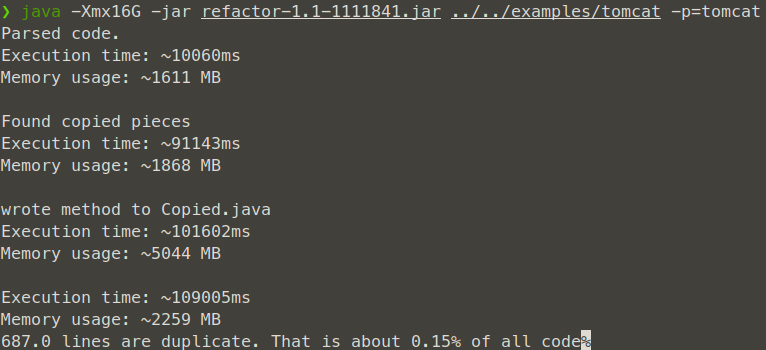
\includegraphics[width=\textwidth]{add3}
    \caption{\centering Приклад обробки більш великого проєкту програмою}
\end{figure} \hfill \\
\section*{Додаток Г}
\begin{figure}[h]
    \centering
    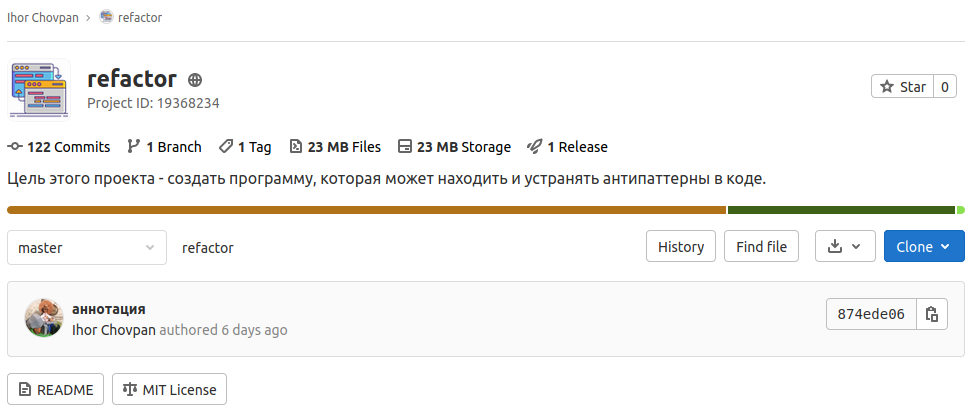
\includegraphics[width=\textwidth]{add-gitlab}
    \caption{\centering Зовнішній вигляд репозиторію програми. \protect\linebreak Посилання: \texttt{gitlab.com/chopikus/refactor} }
\end{figure} \hfill \\

\end{document}
